\chapter{Concepts \& Documentation}

\section*{What is ERP?}
Enterprise Resource Planning (ERP) is a system that integrates business functions into a unified platform. In the Coffee Chain ERP, ERP connects menu management, sales, customer tracking, and outlet operations to reduce redundancy and increase efficiency.

\section*{ERP Integration in the Coffee Chain}
Data flows seamlessly across modules:
\begin{itemize}
    \item A sale connects menu items, customers, and outlet records automatically.  
    \item Menu updates reflect immediately in sales transactions.  
    \item Customers are linked with sales orders for record-keeping and CRM purposes.
\end{itemize}

\section*{Key Concepts}

\subsection*{Coffee Menu Items}
\begin{itemize}
    \item Name, price, category, description, and status (draft, active, seasonal, retired).  
    \item Customization options: milk type, size, syrup flavor, extra shot.  
    \item Linked to Odoo products to integrate with sales.
\end{itemize}

\subsection*{Outlets}
\begin{itemize}
    \item Stores outlet details, including name, manager, and location.  
    \item Linked to sales orders to track which outlet processed each sale.  
    \item Managers oversee staff and validate transactions.
\end{itemize}

\subsection*{Customers and Sales Orders}
\begin{itemize}
    \item Customers are tracked in the CRM and linked to sales orders.  
    \item Sales orders record menu items sold, outlet, customer, payment, and timestamp.  
    \item Acts as the central point connecting menu items, outlets, and customers.
\end{itemize}

\section*{Important Documents in the Workflow}
\begin{itemize}
    \item \textbf{Menu Master List:} Stores all coffee items with categories, prices, and customization options. Serves as the single reference for all outlets.  
    \item \textbf{Sales Records:} Include transaction ID, menu items sold, outlet, customer, and payment details.  
    \item \textbf{Customer Records:} Store contact details and link to sales orders.  
    \item \textbf{Outlet Data Sheets:} Maintain outlet name, location, and manager information.
\end{itemize}

\section*{Module-Document Integration}
\begin{itemize}
    \item Sales orders link menu items to the outlet and customer.  
    \item Menu master list ensures all outlets use consistent item data.  
    \item Customer records are connected to sales orders for traceability.
\end{itemize}

\begin{lstlisting}[language=Python, caption={Example: Linking Outlet and Customer in Sales Order}]
class SaleOrder(models.Model):
    _inherit = 'sale.order'

    outlet_id = fields.Many2one('coffee.outlet', string='Outlet')
    customer_id = fields.Many2one('res.partner', string='Customer')
\end{lstlisting}

\begin{figure}[H]
\centering
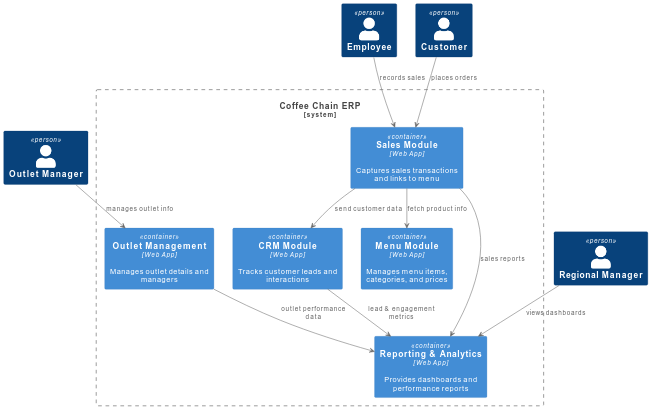
\includegraphics[width=0.9\textwidth,keepaspectratio]{diagrams/C2.png}
\caption{Reference Container Diagram for Module and Document Flow}
\end{figure}

\section*{Insights}
\begin{itemize}
    \item The ERP system connects menu, outlets, customers, and sales orders for seamless operations.  
    \item Centralized documentation ensures consistency across outlets.  
    \item Accurate records of menu items, outlets, and sales orders are essential for reliable operations.  
    \item Maintaining a single source of truth for menu items, outlets, and customers simplifies management and improves traceability.
\end{itemize}
